\documentclass[conference]{IEEEtran}

\usepackage{amsmath,amssymb,amsfonts}
\usepackage{graphicx}
\usepackage{textcomp}
\usepackage{booktabs}
\usepackage{multirow}
\usepackage{xcolor}
\usepackage{hyperref}
\usepackage{float}
\usepackage{array}
\usepackage{tabularx}
\usepackage{caption}
\usepackage{subcaption}
\usepackage{tikz}
\usetikzlibrary{positioning, arrows.meta, shapes.geometric, fit, backgrounds, calc, decorations.pathreplacing}

\hypersetup{colorlinks=true, linkcolor=blue, citecolor=blue, urlcolor=blue}

\begin{document}

\title{Iterative Development of a Kenya Sign Language Recognition System: Lessons from 25 Model Versions}

\author{
\IEEEauthorblockN{Hassan Mahmoud}
\IEEEauthorblockA{University of Colorado Boulder\\Boulder, CO, USA\\hama5612@colorado.edu}
}

\maketitle

% ============================================================
% ABSTRACT
% ============================================================
\begin{abstract}
We document the full iterative development of the first automated recognition system for Kenya Sign Language (KSL), tracing its evolution across 25 model versions that span three architectural paradigms: sequence models, temporal pyramid networks, and spatial-temporal graph convolutional networks. The system recognizes 30 isolated sign classes (15 numbers, 15 words) from hand and upper-body landmarks extracted via MediaPipe Holistic. What started as a bare-bones Transformer prototype grew through CNN-LSTM hybrids with hand-crafted features (peaking at 83.7\% validation), then shifted to a graph convolutional architecture that operates directly on the 48-joint hand-and-body skeleton. Our best overall real-world model (v22)---a 776K-parameter ST-GCN with gradient reversal for signer-invariant learning---reaches 93.3\% validation accuracy, yet only 40.7\% on three unseen signers. Version 25, which introduced hand-to-body spatial features and temporal CutMix, pushed word recognition to a new high of 49.4\% but saw number accuracy collapse to 27.1\%, landing at 38.3\% combined. Leave-one-signer-out cross-validation on v25 yielded 94.7\%, exposing a 56-point gap to real-world performance that we trace squarely to out-of-distribution signer variation. A data audit during v25 development revealed that two of our five training ``signers'' were byte-identical duplicates, meaning we effectively trained on four unique individuals. Across every version tested on real signers (v19--v25), accuracy stays pinned between 30\% and 41\% regardless of architecture. Multi-stream fusion, prototypical classification, MixStyle domain randomization, ArcFace margins, and test-time augmentation all failed to break through. We argue this ceiling is a data diversity problem, not an architectural one, and that honest reporting of this 25-version journey---dead ends and all---serves the field better than cherry-picked final results.
\end{abstract}

\begin{IEEEkeywords}
Kenya Sign Language, graph convolutional networks, sign language recognition, domain generalization, MediaPipe, iterative development
\end{IEEEkeywords}

% ============================================================
% 1. INTRODUCTION
% ============================================================
\section{Introduction}

Roughly 600,000 deaf and hard-of-hearing people in Kenya depend on Kenya Sign Language (KSL) as their primary way of communicating~\cite{ai4ksl2024}. The language has constitutional recognition, but computationally it's almost invisible. American, Chinese, and British Sign Languages have entire research ecosystems built around them; KSL has virtually nothing. That gap matters---it means the communities that need assistive technology the most are the last ones to get it.

Sign language recognition has come a long way from glove-based sensors to vision pipelines built on pose estimation~\cite{robert2023review}. Landmark-based methods, which pull skeletal coordinates out of video frames, handle variations in lighting and background surprisingly well~\cite{aiman2023}. Graph Convolutional Networks~\cite{yan2018stgcn} have become the go-to approach for skeleton-based recognition because they can model joint relationships spatially and track how those relationships change over time. But cross-signer generalization---making a model work on people it's never seen---is still genuinely hard, the sign-language analogue of speaker-independent speech recognition~\cite{pu2024signer, desmond2024}.

There's another problem the field doesn't talk about enough: the gap between what actually happens during development and what shows up in publications. Most papers present a polished final model. The false starts, the techniques that didn't pan out, the bugs that silently corrupted results for weeks---all of that gets left on the cutting room floor~\cite{lipton2019, dodge2019}. It makes the work look cleaner than it was, and it means other researchers end up repeating the same mistakes.

We're taking a different approach here. This paper documents the \textit{entire} iterative development of our KSL recognition system across 25 model versions, spanning three architectural paradigms (Transformers and LSTMs, temporal pyramid CNNs, and graph convolutional networks), two compute platforms (cloud GPU and university HPC cluster), and roughly six months of experimentation. We report every version---the ones that worked and the many that didn't---because we think that's more useful than pretending we nailed it on the first try.

Our contributions:
\begin{enumerate}
    \item The first automated KSL recognition system, establishing a baseline for this under-resourced language.
    \item A complete 25-version development history across three architectural paradigms, serving as a case study in iterative ML system building.
    \item A compact ST-GCN architecture (776K parameters) with gradient reversal that hits 93.3\% validation accuracy.
    \item Evidence of a hard ceiling around 40\% on unseen signers with four training signers, showing that data diversity---not model design---is what's holding us back.
    \item Comprehensive negative results: multi-stream fusion, prototypical networks, MixStyle, ArcFace, hand-body spatial features, temporal CutMix, and test-time augmentation all failed to meaningfully improve cross-signer generalization.
    \item Diagnostic findings from a data audit---including the discovery that two ``different'' training signers were identical files and a MediaPipe version mismatch between training and evaluation data.
\end{enumerate}

% ============================================================
% 2. RELATED WORK
% ============================================================
\section{Related Work}

\subsection{Sign Language Recognition}

The earliest SLR systems applied CNNs to individual frames or short video clips~\cite{pigou2015, oyedotun2017}, then bolted on temporal modeling with RNNs and LSTMs~\cite{hochreiter1997, huang2022}. Koller et al.~\cite{koller2015} showed that CNN-HMM hybrids could handle continuous SLR across multiple signers. More recently, landmark-based pipelines have taken over much of the field: Anithadevi et al.~\cite{anithadevi2025} paired MediaPipe with LSTMs to hit 97\% on 30 Indian Sign Language categories, and Moustafa et al.~\cite{moustafa2023} reached 97.1\% on Arabic Sign Language using MediaPipe and CNNs. Hasan et al.~\cite{hasan2025} reported 94.71\% for Bangla Sign Language with multimodal fusion across 16 signers. The catch is that most of these results come from evaluations where the model has already seen the test signers during training, which makes direct comparison with cross-signer protocols tricky.

\subsection{Graph Convolutional Networks}

Yan et al.~\cite{yan2018stgcn} kicked off the ST-GCN era for skeleton-based action recognition, treating body joints as nodes in a graph. Shi et al.~\cite{shi2019twostreamAGCN} built on that with adaptive graph topologies and a two-stream setup (joints plus bone vectors). Liu et al.~\cite{liu2020msg3d} went further with multi-scale graph convolution, and Chen et al.~\cite{chen2021ctrgcn} introduced channel-wise topology refinement. On the hand gesture side, Aiman and Ahmad~\cite{aiman2023} proposed angle-based GCN features specifically to fight overfitting on small datasets. Our architecture sits in the ST-GCN family, adapted for the 48-node hand-and-upper-body skeleton we settled on after several rounds of experimentation.

\subsection{Kenya Sign Language}

There's almost nothing published on KSL from a computational standpoint. The AI4KSL project~\cite{ai4ksl2024} assembled a MediaPipe-based KSL dataset. Amukasa~\cite{amukasa2021} took a look at CNN-based KSL alphabet recognition. That's about it. The scarcity makes our contribution novel almost by default, though we'd prefer it were novel for the right reasons.

\subsection{Domain Generalization and Signer Independence}

Ganin et al.~\cite{ganin2016domain} introduced the Gradient Reversal Layer for learning domain-invariant features. Pu et al.~\cite{pu2024signer} recast signer-independent SLR as a domain generalization problem, which is how we think about it too. Zhou et al.~\cite{zhou2021mixstyle} proposed MixStyle, which mixes feature statistics across domains during training to encourage generalization. Desmond et al.~\cite{desmond2024} carefully documented the 20--40 percentage point drops in accuracy that come with signer-independent evaluation---numbers that match what we've seen. Snell et al.~\cite{snell2017prototypical} introduced prototypical networks for few-shot classification, and Guo et al.~\cite{guo2024fewshot} got 43.75\% on ASL with prototypical networks, which is actually quite close to where we ended up.

\subsection{Training Methodology}

Our training pipeline draws on a well-established toolbox: AdamW with decoupled weight decay~\cite{loshchilov2019adamw}, cosine annealing schedules~\cite{loshchilov2017cosine}, batch normalization~\cite{ioffe2015}, dropout~\cite{srivastava2014}, label smoothing~\cite{szegedy2016, muller2019}, focal loss for class imbalance~\cite{lin2017focal}, and supervised contrastive learning~\cite{khosla2020supcon}. For skeleton-specific augmentations, we followed standard practices: rotation, scaling, jittering, and temporal warping~\cite{kolawole2024augmentation}.

\subsection{Evaluation Methodology}

Li et al.~\cite{li2020wlasl} and Sincan and Keles~\cite{sincan2020autsl} established signer-independent evaluation protocols that consistently show much lower accuracy than same-signer testing. We adopted this stricter protocol from the start and, following the arguments of Lipton and Steinhardt~\cite{lipton2019} and Dodge et al.~\cite{dodge2019}, committed to reporting everything---including the experiments that went nowhere.

% ============================================================
% 3. SYSTEM OVERVIEW
% ============================================================
\section{System Overview}

\subsection{Task Definition}

We tackle isolated sign recognition across 30 KSL classes: 15 numbers (9, 17, 22, 35, 48, 54, 66, 73, 89, 91, 100, 125, 268, 388, 444) and 15 words (Agreement, Apple, Colour, Friend, Gift, Market, Monday, Picture, Proud, Sweater, Teach, Tomatoes, Tortoise, Twin, Ugali). Each sign is a single, self-contained gesture captured on video.

\subsection{Data Collection}

Videos came from native KSL signers, with roughly 5 repetitions of each sign per signer. After deduplication, the training set has about 250 samples per category from what we initially believed were 5 signers. A data audit during v25 development uncovered something we hadn't expected: two of those signers (signers 2 and 3) turned out to be byte-for-byte identical files. So we effectively trained on 4 unique signers, not 5. The validation set is 360 samples from a held-out signer who was recorded under the same conditions as training. Starting at v19, we also collected 140 real-world videos (59 numbers, 81 words) from three entirely new signers recorded in naturalistic settings.

\subsection{Landmark Extraction}

MediaPipe Holistic (v0.10.14 for training data) extracts 549 dimensions per frame: 33 pose landmarks, 21 left-hand landmarks, 21 right-hand landmarks, 68 face keypoints, and 40 lip points. Early versions consumed all 549 features, but we eventually settled on 48 selected nodes (42 hand joints plus 6 upper-body pose landmarks) for the GCN-based architectures. It's worth noting that our real-world evaluation data was processed with MediaPipe v0.10.5---a version mismatch we only identified during the v25 diagnostic audit.

% ============================================================
% 4. ARCHITECTURAL EVOLUTION
% ============================================================
\section{Architectural Evolution}

The system went through three distinct architectural paradigms across 25 versions, summarized in Table~\ref{tab:full_evolution} and traced in Fig.~\ref{fig:timeline}.

\begin{figure}[t]
    \centering
    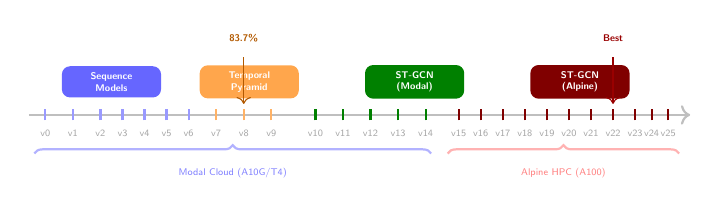
\begin{tikzpicture}[scale=0.7, transform shape,
        era/.style={rectangle, rounded corners=3pt, minimum height=0.5cm, font=\tiny\sffamily\bfseries, text=white, minimum width=1.8cm, align=center},
        ver/.style={font=\tiny\sffamily, text=gray!70},
        milestone/.style={font=\tiny\sffamily\bfseries},
    ]
    % Timeline arrow
    \draw[thick, ->, gray!50] (0, 0) -- (12.0, 0);

    % Era blocks
    \node[era, fill=blue!60] at (1.5, 0.6) {Sequence\\Models};
    \node[era, fill=orange!70] at (4.0, 0.6) {Temporal\\Pyramid};
    \node[era, fill=green!50!black] at (7.0, 0.6) {ST-GCN\\(Modal)};
    \node[era, fill=red!50!black] at (10.0, 0.6) {ST-GCN\\(Alpine)};

    % Version markers
    \foreach \x/\v in {0.3/v0, 0.8/v1, 1.3/v2, 1.7/v3, 2.1/v4, 2.5/v5, 2.9/v6} {
        \draw[blue!40, thick] (\x, -0.1) -- (\x, 0.1);
        \node[ver, below] at (\x, -0.15) {\v};
    }
    \foreach \x/\v in {3.4/v7, 3.9/v8, 4.4/v9} {
        \draw[orange!60, thick] (\x, -0.1) -- (\x, 0.1);
        \node[ver, below] at (\x, -0.15) {\v};
    }
    \foreach \x/\v in {5.2/v10, 5.7/v11, 6.2/v12, 6.7/v13, 7.2/v14} {
        \draw[green!50!black, thick] (\x, -0.1) -- (\x, 0.1);
        \node[ver, below] at (\x, -0.15) {\v};
    }
    \foreach \x/\v in {7.8/v15, 8.2/v16, 8.6/v17, 9.0/v18, 9.4/v19, 9.8/v20, 10.2/v21, 10.6/v22, 11.0/v23, 11.3/v24, 11.6/v25} {
        \draw[red!50!black, thick] (\x, -0.1) -- (\x, 0.1);
        \node[ver, below] at (\x, -0.15) {\v};
    }

    % Key milestones
    \node[milestone, above=0.3cm, text=orange!70!black] at (3.9, 0.9) {83.7\%};
    \node[milestone, above=0.3cm, text=red!60!black] at (10.6, 0.9) {Best};
    \draw[->, thin, orange!70!black] (3.9, 1.05) -- (3.9, 0.2);
    \draw[->, thin, red!60!black] (10.6, 1.05) -- (10.6, 0.2);

    % Platform labels
    \draw[decorate, decoration={brace, amplitude=3pt}, thick, blue!30]
        (0.1, -0.7) -- (7.3, -0.7) node[midway, below=4pt, font=\tiny\sffamily, text=blue!50] {Modal Cloud (A10G/T4)};
    \draw[decorate, decoration={brace, amplitude=3pt}, thick, red!30]
        (7.6, -0.7) -- (11.8, -0.7) node[midway, below=4pt, font=\tiny\sffamily, text=red!50] {Alpine HPC (A100)};

    \end{tikzpicture}
    \caption{Development timeline across 25 versions and three architectural paradigms. v8 achieved the best pre-real-tester validation (83.7\%); v22 achieved the best real-world accuracy (40.7\%); v25 achieved the best word recognition (49.4\%).}
    \label{fig:timeline}
\end{figure}

\subsection{Phase 1: Sequence Models (v0--v6)}

We started with what seemed reasonable at the time: a minimal 2-layer Transformer encoder operating on 225 raw landmark features (pose plus both hands) with nothing but Gaussian noise for augmentation. That was v0. Version 1 scaled it up---a 4-layer Transformer and 3-layer bidirectional LSTM with attention, adding AdamW and basic augmentations (noise, time shift, scaling). By v2, we were already worried about overfitting, so we shrank the model, cranked weight decay up to 0.05, and introduced cosine annealing with warmup.

Then things got complicated. Version 3 tripled the input dimension from 225 to 801 by computing velocity and acceleration features, and threw in focal loss, stochastic weight averaging, test-time augmentation, and model ensembling. Version 4 added face and lip landmarks (549 total features), built a body-part attention mechanism that processed pose, hands, and face through separate streams, and introduced a CNN-Transformer hybrid architecture. Version 5 went deep on hand-specific feature engineering---finger angles, fingertip distances, curl measurements, palm normals---pushing the feature count to 649. Version 6 tried supervised contrastive learning, which actually hurt classification accuracy and was promptly dropped.

Looking back, the whole phase was handicapped by one thing: we were treating the hand as a flat feature vector instead of what it actually is---a structured graph of connected joints. We also didn't have systematic validation tracking, so we were flying partially blind.

\subsection{Phase 2: Temporal Pyramid Networks (v7--v9)}

Version 7 marked a real shift in approach: a Temporal Pyramid architecture with multi-scale 1D convolutions (kernels 3, 7, 15) feeding a 3-layer bidirectional LSTM with 4-head attention. It ran on the 649 hand-engineered features and used focal loss with 3$\times$ weight boosting on the hardest classes (444 and 35). Validation climbed to about 80\%, but class 54 became a serious problem---it acted like a black hole, pulling predictions from multiple other classes toward it.

Version 8 tried to fix this head-on with a confusion-aware loss function that specifically penalized 9 known confusion pairs, plus a dedicated anti-attractor head targeting class 54. That got us to \textbf{83.7\% combined validation accuracy}---the best result of the pre-Alpine era. It would take 14 more versions to beat it convincingly. Version 9 tacked on 8 temporal segmentation features (duration statistics, velocity profiles, gesture peak counts), but the confusion-penalty approach was hitting diminishing returns by this point.

\subsection{Phase 3: Graph Convolutional Networks on Modal (v10--v14)}

Version 10 was the biggest bet of the whole project. We scrapped the entire feature-engineering pipeline and replaced it with a 6-layer ST-GCN~\cite{yan2018stgcn} operating directly on raw $(x,y,z)$ coordinates of 42 hand joints. Every one of those 100-plus engineered features---gone, just like that. The gamble was that the GCN could learn spatial hand relationships from the graph structure alone. Version 11 split the single 30-class model into two separate 15-class models for numbers and words, a design decision we've kept ever since.

Version 12 grew the graph to 48 nodes by bringing in 6 upper-body pose joints (shoulders, elbows, wrists) for arm context. Versions 13 and 14 pushed into territory that, in retrospect, was reckless: extremely aggressive hand landmark dropout, zeroing out up to 90\% of joints during training. Our reasoning was that forcing the model to recognize signs from partial skeletons would build robustness. It didn't---it destroyed number recognition, as we'd painfully discover in v15.

\subsection{Phase 4: Alpine HPC Era (v15--v18)}

Moving to the Alpine HPC cluster (University of Colorado Boulder) for v15 gave us our first proper validation numbers: 48.9\% for numbers, 89.7\% for words, 69.3\% combined. That 40-point gap between numbers and words told the story plainly: the extreme hand dropout from v13--v14 was stripping out exactly the fine-grained shape information that number signs need.

Version 16 was an exercise in throwing everything at the wall. Confusion-aware focal loss, an anti-attractor head, supervised contrastive learning, mixup---we reintroduced most of the complexity we'd removed in v10. Class 444 jumped from 0\% to 45\%, but class 66 went the other direction (92\% down to 36\%). Net result: 69.4\% combined. We'd shuffled the errors around without actually reducing them.

Version 17 took the opposite tack. We stripped everything back to the bare ST-GCN with standard cross-entropy loss. Combined accuracy: 72.6\%---the best Alpine result yet. The lesson was hard to miss: simplification beat sophistication. On top of that, a thorough pipeline audit turned up 4 bugs we didn't know we had---normalization squashing, dead SWA code that was never executing, a temporal roll that wrapped around incorrectly, and an incomplete hand-swap augmentation.

Version 18 fixed 11 bugs total, added velocity features (6 input channels), and swapped in 2-head attention pooling. Validation actually dropped to 70.6\%, probably because of complex interactions between the newly fixed code paths. But this version laid the groundwork---velocity features, attention pooling, a bug-free pipeline---that made everything after v19 possible.

\subsection{Phase 5: Real-World Evaluation Era (v19--v25)}

Starting with v19, we began evaluating on three signers who had never appeared in training or validation. This was the moment that fundamentally changed how we thought about our models. Version 19 looked great on validation (87.3\%) but scored just 34.2\% on real testers---a 53-point gap that had been completely invisible before.

Version 20 tried aggressive file-level deduplication, which accidentally removed useful training variation (86.9\% val, 30.3\% real---actually worse). Version 21 introduced ArcFace angular margin loss~\cite{deng2019arcface}, and it was, frankly, a disaster: 76.5\% validation, 31.2\% real. ArcFace needs diverse training examples to learn meaningful margins, and four signers simply wasn't enough.

\textbf{Version 22} is still our best overall real-world model. We removed ArcFace, turned the GRL up to $\lambda_{\max}=0.3$, dialed back augmentation aggressiveness, added bone vector features (bringing input to 9 channels), and introduced supervised contrastive loss with signer-balanced batch sampling. At 776K parameters and just 7.3 minutes of training, it reached 93.3\% validation and \textbf{40.7\% combined real-world accuracy} (33.9\% numbers, 45.7\% words). Not spectacular in absolute terms, but it was the first model to crack 40\%.

Version 23 went big---four independent streams (joint, bone, velocity, bone velocity) with focal loss and grid-searched fusion weights. Validation hit a record 95.6\%, which was exciting until we ran the real-tester evaluation: 38.6\%. The joint stream alone matched the fused result, and stream agreement was dismal (19\% for numbers, 30\% for words). Four correlated views of the same limited data don't add up to a better result.

Version 24 tried prototypical classification with MixStyle domain randomization. Words hit 49.4\%---the best we'd ever seen---but numbers cratered to 25.4\%, the worst ever. Combined: 39.3\%. The prototypical classifier performed identically to a standard FC head, confirming our growing suspicion that the features themselves were the bottleneck, not how we classified them.

\textbf{Version 25} explored a hypothesis that came out of a diagnostic audit: our wrist-centric normalization was throwing away potentially valuable information about where the hands were relative to the body. We added 8 hand-to-body spatial features---hand height relative to shoulders, lateral hand position, hand-to-face distance, inter-hand distance, and a symmetry measure---all computed \textit{before} the normalization step that would otherwise discard this information. We also introduced temporal CutMix~\cite{zhang2018mixup} ($\alpha=1.0$, $p=0.3$), applied as a mutually exclusive alternative to Mixup during training.

The results told a split story. Words reached \textbf{49.4\%}---tying v24 for the best we've ever achieved---which made sense because many word signs involve distinctive body locations (signing near the face vs.\ at chest height). But numbers collapsed to 27.1\%, worse than any previous version. Number signs rely on hand shape, not body-relative position, so the extra spatial features were apparently acting as noise. Combined accuracy landed at 38.3\%, below v22's 40.7\%.

To get a better handle on whether the model was genuinely learning or just memorizing our four signers, we ran leave-one-signer-out (LOSO) cross-validation on v25: numbers 92.4\%$\pm$5.4\%, words 97.1\%$\pm$2.6\%, combined 94.7\%. Compare that to the 38.3\% we got on actual new signers. That 56.4-point gap---between LOSO and real-world---tells us the model transfers beautifully within the training distribution but falls apart on genuinely out-of-distribution signers.

During the v25 development cycle, a routine data audit turned up two surprises. First, signers 2 and 3 in our training set produced identical MD5 hashes---they were byte-for-byte duplicate files. What we'd thought was a 5-signer training set was really 4 unique signers. Second, we discovered that the training data had been extracted with MediaPipe v0.10.14 while our real-world evaluation pipeline used v0.10.5. Minor version differences in MediaPipe can shift landmark coordinates slightly, adding noise to what's already a difficult cross-signer evaluation.

% ============================================================
% 5. BEST MODEL ARCHITECTURE (v22)
% ============================================================
\section{Best Model Architecture}

The best real-world model (v22) is described below and illustrated in Figs.~\ref{fig:skeleton} and~\ref{fig:architecture}.

\begin{figure}[t]
    \centering
    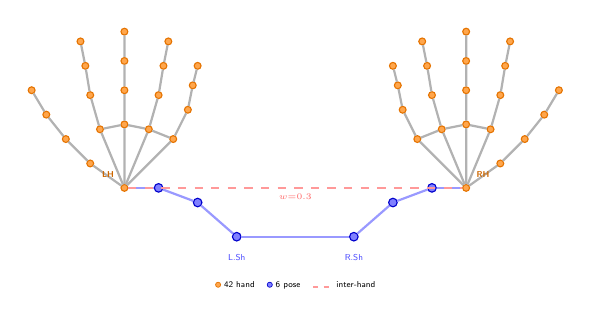
\begin{tikzpicture}[
        scale=0.62, transform shape,
        joint/.style={circle, fill=orange!70, draw=orange!90!black, inner sep=0pt, minimum size=4pt},
        pose/.style={circle, fill=blue!50, draw=blue!80!black, inner sep=0pt, minimum size=5pt},
        edge/.style={thick, gray!60},
        poseedge/.style={thick, blue!40},
        interhand/.style={thick, dashed, red!40},
    ]
    % LEFT HAND
    \node[joint] (lw) at (-3.5, 0) {};
    \node[joint] (l1) at (-4.2, 0.5) {}; \node[joint] (l2) at (-4.7, 1.0) {};
    \node[joint] (l3) at (-5.1, 1.5) {}; \node[joint] (l4) at (-5.4, 2.0) {};
    \node[joint] (l5) at (-4.0, 1.2) {}; \node[joint] (l6) at (-4.2, 1.9) {};
    \node[joint] (l7) at (-4.3, 2.5) {}; \node[joint] (l8) at (-4.4, 3.0) {};
    \node[joint] (l9) at (-3.5, 1.3) {}; \node[joint] (l10) at (-3.5, 2.0) {};
    \node[joint] (l11) at (-3.5, 2.6) {}; \node[joint] (l12) at (-3.5, 3.2) {};
    \node[joint] (l13) at (-3.0, 1.2) {}; \node[joint] (l14) at (-2.8, 1.9) {};
    \node[joint] (l15) at (-2.7, 2.5) {}; \node[joint] (l16) at (-2.6, 3.0) {};
    \node[joint] (l17) at (-2.5, 1.0) {}; \node[joint] (l18) at (-2.2, 1.6) {};
    \node[joint] (l19) at (-2.1, 2.1) {}; \node[joint] (l20) at (-2.0, 2.5) {};
    \foreach \a/\b in {lw/l1,l1/l2,l2/l3,l3/l4,lw/l5,l5/l6,l6/l7,l7/l8,lw/l9,l9/l10,l10/l11,l11/l12,lw/l13,l13/l14,l14/l15,l15/l16,lw/l17,l17/l18,l18/l19,l19/l20,l5/l9,l9/l13,l13/l17}
        \draw[edge] (\a) -- (\b);
    % RIGHT HAND
    \node[joint] (rw) at (3.5, 0) {};
    \node[joint] (r1) at (4.2, 0.5) {}; \node[joint] (r2) at (4.7, 1.0) {};
    \node[joint] (r3) at (5.1, 1.5) {}; \node[joint] (r4) at (5.4, 2.0) {};
    \node[joint] (r5) at (4.0, 1.2) {}; \node[joint] (r6) at (4.2, 1.9) {};
    \node[joint] (r7) at (4.3, 2.5) {}; \node[joint] (r8) at (4.4, 3.0) {};
    \node[joint] (r9) at (3.5, 1.3) {}; \node[joint] (r10) at (3.5, 2.0) {};
    \node[joint] (r11) at (3.5, 2.6) {}; \node[joint] (r12) at (3.5, 3.2) {};
    \node[joint] (r13) at (3.0, 1.2) {}; \node[joint] (r14) at (2.8, 1.9) {};
    \node[joint] (r15) at (2.7, 2.5) {}; \node[joint] (r16) at (2.6, 3.0) {};
    \node[joint] (r17) at (2.5, 1.0) {}; \node[joint] (r18) at (2.2, 1.6) {};
    \node[joint] (r19) at (2.1, 2.1) {}; \node[joint] (r20) at (2.0, 2.5) {};
    \foreach \a/\b in {rw/r1,r1/r2,r2/r3,r3/r4,rw/r5,r5/r6,r6/r7,r7/r8,rw/r9,r9/r10,r10/r11,r11/r12,rw/r13,r13/r14,r14/r15,r15/r16,rw/r17,r17/r18,r18/r19,r19/r20,r5/r9,r9/r13,r13/r17}
        \draw[edge] (\a) -- (\b);
    % POSE
    \node[pose] (ls) at (-1.2, -1.0) {}; \node[pose] (rs) at (1.2, -1.0) {};
    \node[pose] (le) at (-2.0, -0.3) {}; \node[pose] (re) at (2.0, -0.3) {};
    \node[pose] (lwrist) at (-2.8, 0.0) {}; \node[pose] (rwrist) at (2.8, 0.0) {};
    \draw[poseedge] (ls)--(rs); \draw[poseedge] (ls)--(le); \draw[poseedge] (rs)--(re);
    \draw[poseedge] (le)--(lwrist); \draw[poseedge] (re)--(rwrist);
    \draw[poseedge] (lwrist)--(lw); \draw[poseedge] (rwrist)--(rw);
    \draw[interhand] (lw) -- (rw) node[midway, below, font=\tiny, text=red!60] {$w$=0.3};
    \node[font=\tiny\sffamily, below=0.15cm of ls, text=blue!70] {L.Sh};
    \node[font=\tiny\sffamily, below=0.15cm of rs, text=blue!70] {R.Sh};
    \node[font=\tiny\sffamily, above left=0.05cm of lw, text=orange!80!black] {\textbf{LH}};
    \node[font=\tiny\sffamily, above right=0.05cm of rw, text=orange!80!black] {\textbf{RH}};
    \node[font=\tiny\sffamily] at (0, -2.0) {
        \tikz{\node[joint,minimum size=3pt] {};} 42 hand \quad
        \tikz{\node[pose,minimum size=3pt] {};} 6 pose \quad
        \tikz{\draw[interhand,thick] (0,0)--(0.4,0);} inter-hand};
    \end{tikzpicture}
    \caption{48-node skeleton graph. Hands (orange, 21 joints each) connect via finger kinematic chains; 6 pose joints (blue) provide upper-body context; a weak inter-hand edge (dashed) links wrists.}
    \label{fig:skeleton}
\end{figure}

\subsection{Preprocessing}

Each frame gets normalized per body segment: hands are centered at the wrist and scaled by palm size, while pose is centered at mid-shoulder and scaled by shoulder width. We compute 9 input channels: raw joint coordinates $(x,y,z)$, temporal velocity ($v_t = h_t - h_{t-1}$), and bone vectors (parent-to-child displacements). An auxiliary branch receives 53 features---33 joint angles and 20 pairwise fingertip distances. All videos are resampled to $T=90$ frames, yielding tensors of shape $(9, 90, 48)$ for the main branch and $(90, 53)$ for the auxiliary.

\subsection{Architecture}

The model has four main pieces: a 4-layer ST-GCN backbone (channels $[9, 64, 64, 128, 128]$, multi-scale temporal convolutions with kernels $\{3, 5, 7\}$, spatial node dropout at $p=0.1$, temporal stride of 2 at layers 1 and 3), a 2-head temporal attention pooling layer producing a 256-dimensional GCN embedding, an auxiliary branch (MLP followed by Conv1D followed by attention pooling, outputting 64 dimensions), and a classification head that operates on the concatenated 320-dimensional embedding. A Gradient Reversal Layer~\cite{ganin2016domain} feeds a signer discrimination head, with $\lambda$ ramped linearly from 0 to 0.3 over 100 epochs to encourage signer-invariant feature learning.

\begin{figure*}[t]
    \centering
    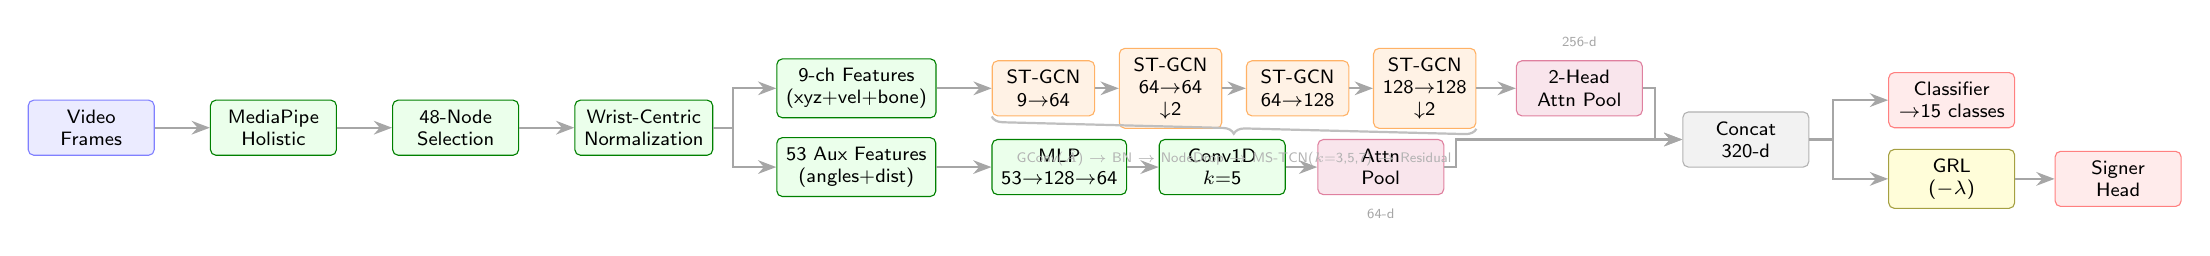
\begin{tikzpicture}[
        node distance=0.5cm and 0.6cm, >=Stealth,
        block/.style={rectangle, draw, rounded corners=2pt, minimum height=0.7cm, minimum width=1.6cm, align=center, font=\scriptsize\sffamily},
        input/.style={block, fill=blue!8, draw=blue!50},
        process/.style={block, fill=green!8, draw=green!50!black},
        gcnblock/.style={block, fill=orange!10, draw=orange!60, minimum width=1.3cm},
        pool/.style={block, fill=purple!10, draw=purple!50},
        head/.style={block, fill=red!8, draw=red!50},
        grl/.style={block, fill=yellow!15, draw=yellow!60!black},
        embed/.style={block, fill=gray!10, draw=gray!60},
        arrow/.style={->, thick, draw=gray!70},
        label/.style={font=\tiny\sffamily, text=gray!70},
    ]
    \node[input] (video) {Video\\Frames};
    \node[process, right=0.7cm of video] (mp) {MediaPipe\\Holistic};
    \node[process, right=0.7cm of mp] (select) {48-Node\\Selection};
    \node[process, right=0.7cm of select] (norm) {Wrist-Centric\\Normalization};
    \node[process, right=0.8cm of norm, yshift=0.5cm] (feat9) {9-ch Features\\(xyz+vel+bone)};
    \node[process, right=0.8cm of norm, yshift=-0.5cm] (feat53) {53 Aux Features\\(angles+dist)};
    \node[gcnblock, right=0.7cm of feat9] (gcn1) {ST-GCN\\9$\to$64};
    \node[gcnblock, right=0.3cm of gcn1] (gcn2) {ST-GCN\\64$\to$64\\$\downarrow$2};
    \node[gcnblock, right=0.3cm of gcn2] (gcn3) {ST-GCN\\64$\to$128};
    \node[gcnblock, right=0.3cm of gcn3] (gcn4) {ST-GCN\\128$\to$128\\$\downarrow$2};
    \node[pool, right=0.5cm of gcn4] (attn) {2-Head\\Attn Pool};
    \node[process, right=0.7cm of feat53] (mlp) {MLP\\53$\to$128$\to$64};
    \node[process, right=0.4cm of mlp] (conv1d) {Conv1D\\$k$=5};
    \node[pool, right=0.4cm of conv1d] (auxpool) {Attn\\Pool};
    \node[embed, right=0.5cm of attn, yshift=-0.65cm] (concat) {Concat\\320-d};
    \node[label, above=0.05cm of attn] {256-d};
    \node[label, below=0.05cm of auxpool] {64-d};
    \node[head, right=1.0cm of concat, yshift=0.5cm] (cls) {Classifier\\$\to$15 classes};
    \node[grl, right=1.0cm of concat, yshift=-0.5cm] (grl) {GRL\\($-\lambda$)};
    \node[head, right=0.5cm of grl] (signer) {Signer\\Head};
    \draw[arrow] (video)--(mp); \draw[arrow] (mp)--(select); \draw[arrow] (select)--(norm);
    \draw[arrow] (norm.east)--++(0.25,0)|-(feat9.west);
    \draw[arrow] (norm.east)--++(0.25,0)|-(feat53.west);
    \draw[arrow] (feat9)--(gcn1); \draw[arrow] (gcn1)--(gcn2);
    \draw[arrow] (gcn2)--(gcn3); \draw[arrow] (gcn3)--(gcn4); \draw[arrow] (gcn4)--(attn);
    \draw[arrow] (feat53)--(mlp); \draw[arrow] (mlp)--(conv1d); \draw[arrow] (conv1d)--(auxpool);
    \draw[arrow] (attn.east)--++(0.15,0)|-(concat.west);
    \draw[arrow] (auxpool.east)--++(0.15,0)|-(concat.west);
    \draw[arrow] (concat.east)--++(0.3,0)|-(cls.west);
    \draw[arrow] (concat.east)--++(0.3,0)|-(grl.west);
    \draw[arrow] (grl)--(signer);
    \draw[decorate, decoration={brace, amplitude=4pt, mirror}, thick, gray!50]
        (gcn1.south west)--(gcn4.south east)
        node[midway, below=6pt, font=\tiny\sffamily, text=gray!60, align=center] {GConv($\hat{A}$) $\to$ BN $\to$ NodeDrop $\to$ MS-TCN($k$=3,5,7) $\to$ Residual};
    \end{tikzpicture}
    \caption{Architecture of the best model (v22). The ST-GCN backbone processes 9-channel skeleton features through 4 graph convolution blocks. An auxiliary branch captures geometric features. The GRL encourages signer-invariant representations.}
    \label{fig:architecture}
\end{figure*}

\subsection{Training}

The loss function combines cross-entropy (label smoothing $\epsilon=0.1$), supervised contrastive loss~\cite{khosla2020supcon} ($\tau=0.07$, weight 0.1), and adversarial signer loss (weight $\lambda$). We train with AdamW~\cite{loshchilov2019adamw} ($\text{lr}=10^{-3}$, weight decay $10^{-3}$), cosine annealing~\cite{loshchilov2017cosine} ($T_{\max}=200$), a 10-epoch warmup, gradient clipping at max norm 1.0, batch size 32, and Mixup~\cite{zhang2018mixup} ($\alpha=0.2$). Twelve augmentation operations run during training, covering temporal and spatial perturbations, hand swaps, bone-length scaling, rotation, and noise injection.

% ============================================================
% 6. RESULTS
% ============================================================
\section{Results}

\subsection{Complete Version Summary}

Table~\ref{tab:full_evolution} lays out the full development history. We didn't track validation results systematically before v15, and real-tester evaluation only started at v19.

\begin{table*}[t]
\centering
\caption{Complete model evolution across 25 versions. Val = validation combined accuracy. Real = real-world combined accuracy on unseen signers (available from v19). Best results per column in \textbf{bold}. Dashes indicate unavailable data.}
\label{tab:full_evolution}
\small
\begin{tabular}{@{}clllcccc@{}}
\toprule
\textbf{Ver} & \textbf{Architecture} & \textbf{Key Change} & \textbf{Platform} & \textbf{Params} & \textbf{Val \%} & \textbf{Real \%} & \textbf{Gap} \\
\midrule
\multicolumn{8}{l}{\textit{Phase 1: Sequence Models}} \\
v0  & 2L Transformer        & Minimal baseline           & Modal A10G & $\sim$100K & --- & --- & --- \\
v1  & 4L Transformer / BiLSTM & Unified 30-class, attention & Modal A10G & $\sim$0.5--1M & --- & --- & --- \\
v2  & 2L Transformer / BiLSTM & Heavy regularization       & Modal A10G & $\sim$300K & --- & --- & --- \\
v3  & Transformer+LSTM ens.  & Vel+accel features, SWA, TTA & Modal A10G & $\sim$500K & --- & --- & --- \\
v4  & CNN+Transformer hybrid & Face/lips, body-part attn  & Modal A10G & $\sim$1--2M & --- & --- & --- \\
v5  & LSTM (number-focused)  & Hand feature engineering    & Modal A10G & $\sim$1M & --- & --- & --- \\
v6  & Contrastive encoder    & SupCon (hurt accuracy)     & Modal A10G & $\sim$500K & --- & --- & --- \\
\midrule
\multicolumn{8}{l}{\textit{Phase 2: Temporal Pyramid Networks}} \\
v7  & Temporal Pyramid+BiLSTM & Focal loss, class boosting & Modal A10G & $\sim$4--5M & $\sim$80 & --- & --- \\
v8  & +Anti-attractor head   & Confusion-aware loss       & Modal A10G & $\sim$4--5M & \textbf{83.7} & --- & --- \\
v9  & +Temporal segmentation & 8 temporal features        & Modal A10G & $\sim$4--5M & $\sim$83 & --- & --- \\
\midrule
\multicolumn{8}{l}{\textit{Phase 3: ST-GCN (Modal Cloud)}} \\
v10 & 6L ST-GCN (42 nodes)   & GCN architecture shift     & Modal A10G & $\sim$1.5--2M & --- & --- & --- \\
v11 & ST-GCN split models    & Separate num/word models   & Modal A10G & $\sim$695K$\times$2 & --- & --- & --- \\
v12 & ST-GCN + 6 pose joints & 48-node graph              & Modal A10G & $\sim$700K$\times$2 & --- & --- & --- \\
v13 & ST-GCN + dropout       & Aggressive landmark dropout & Modal A10G & $\sim$700K$\times$2 & --- & --- & --- \\
v14 & ST-GCN + extreme drop  & 50--90\% hand dropout      & Modal T4   & $\sim$700K$\times$2 & --- & --- & --- \\
\midrule
\multicolumn{8}{l}{\textit{Phase 4: ST-GCN (Alpine HPC)}} \\
v15 & ST-GCN (port of v14)   & First Alpine run           & Alpine L40 & 6.95M & 69.3 & --- & --- \\
v16 & ST-GCN + confusion-aware & Focal+contrastive+anti-attr & Alpine L40 & 2.5/7.0M & 69.4 & --- & --- \\
v17 & ST-GCN simplified      & Removed all complexity     & Alpine A100 & 6.95M$\times$2 & 72.6 & --- & --- \\
v18 & ST-GCN + velocity+attn & 11 bug fixes, 6ch input    & Alpine A100 & 7.3M$\times$2 & 70.6 & --- & --- \\
\midrule
\multicolumn{8}{l}{\textit{Phase 5: Real-World Evaluation}} \\
v19 & ST-GCN + ArcFace stg2 & First real-tester eval      & Alpine A100 & 17.3M & 87.3 & 34.2 & 53.1 \\
v20 & ST-GCN + dedup         & Aggressive deduplication    & Alpine A100 & 827K  & 86.9 & 30.3 & 56.6 \\
v21 & ST-GCN + ArcFace full  & ArcFace (catastrophic)     & Alpine A100 & 1.47M & 76.5 & 31.2 & 45.3 \\
v22 & \textbf{ST-GCN + GRL}  & \textbf{No ArcFace, strong GRL} & Alpine A100 & \textbf{776K$\times$2} & 93.3 & \textbf{40.7} & 52.6 \\
v23 & 4-stream fusion        & Multi-stream + focal loss  & Alpine A100 & 3.1M$\times$2 & \textbf{95.6} & 38.6 & 57.0 \\
v24 & ST-GCN + prototypical  & MixStyle + proto classifier & Alpine A100 & 776K$\times$2 & 91.5 & 39.3 & 52.2 \\
v25 & ST-GCN + hand-body     & Hand-body features + CutMix & Alpine A100 & 777K$\times$2 & 89.1 & 38.3 & 50.8 \\
\bottomrule
\end{tabular}
\end{table*}

\subsection{Real-World Evaluation (v19--v25)}

Table~\ref{tab:real_results} breaks down real-world performance across the seven versions we've tested on unseen signers. The numbers are sobering.

\begin{table}[t]
\centering
\caption{Real-world accuracy on unseen signers (v19--v25). Best per column in \textbf{bold}.}
\label{tab:real_results}
\small
\begin{tabular}{@{}lcccc@{}}
\toprule
\textbf{Ver} & \textbf{Num \%} & \textbf{Words \%} & \textbf{Comb \%} & \textbf{Config} \\
\midrule
v19 & 20.3 & 48.1 & 34.2 & no TTA \\
v20 & 18.6 & 42.0 & 30.3 & no TTA \\
v21 & 25.4 & 37.0 & 31.2 & --- \\
v22 & \textbf{33.9} & 45.7 & \textbf{40.7} & no TTA \\
v23 & \textbf{33.9} & 42.0 & 38.6 & no TTA \\
v24 & 25.4 & \textbf{49.4} & 39.3 & FC head \\
v25 & 27.1 & \textbf{49.4} & 38.3 & no TTA \\
\bottomrule
\end{tabular}
\end{table}

\subsection{Leave-One-Signer-Out Cross-Validation (v25)}

To assess how well our architecture generalizes within the training distribution, we ran LOSO cross-validation on v25. With 4 unique training signers (after accounting for the discovered duplicates), this is a 4-fold setup. Results: numbers 92.4\%$\pm$5.4\%, words 97.1\%$\pm$2.6\%, combined 94.7\%. The 56.4-point gap between LOSO (94.7\%) and real-world (38.3\%) performance starkly illustrates the out-of-distribution nature of the signer generalization problem. LOSO is useful as a sanity check---it confirms the model architecture can learn the task---but it doesn't predict real-world accuracy on genuinely new signers.

\subsection{Ablation Studies}

\subsubsection{Test-Time Augmentation (v22, v25)}
TTA (averaging predictions over 5 augmented copies of each input) consistently hurts. In v22, it dropped accuracy by 1.4pp overall---numbers fell 5.1pp while words gained a mere 1.2pp. In v25, TTA reduced combined accuracy by 1.2pp. We disabled it from v23 onward and don't plan to revisit it.

\subsubsection{Multi-Stream Fusion (v23)}
We trained four independent streams and measured per-stream real accuracy: joint 37.3\%/42.0\%, bone 33.9\%/42.0\%, velocity 30.5\%/37.0\%, bone-velocity 35.6\%/39.5\% (numbers/words). The fused result (33.9\%/42.0\%) couldn't outperform the best single stream. Stream agreement was low---18.6\% for numbers and 29.6\% for words had all four streams agree---but the streams weren't making \textit{complementary} errors. They were making the same kinds of mistakes on the same hard examples.

\subsubsection{Hand-Body Spatial Features (v25)}
Eight features capturing hand position relative to the body (hand height, lateral position, hand-to-face distance, inter-hand distance, symmetry) were computed before wrist-centric normalization. These helped words (+3.7pp vs v22) because word signs often involve distinctive body locations. They hurt numbers ($-$6.8pp vs v22) because number signs depend on hand shape, not where the hand is in space. The features added signal for one task and noise for the other.

\subsubsection{Temporal CutMix (v25)}
CutMix ($\alpha=1.0$, $p=0.3$), which splices random temporal segments between training examples, was applied as a mutually exclusive alternative to Mixup. Its effect couldn't be cleanly isolated from the hand-body features since both were introduced in v25, but the combined result didn't improve on v22.

\subsubsection{Prototypical Classification (v24)}
Cosine-similarity-based classification against class prototypes ($\tau=0.1$) performed identically to a standard FC head: 25.4\% numbers and 48.1\% vs 49.4\% words. Same features in, same results out. MixStyle didn't help either.

\subsubsection{ArcFace (v21)}
Angular margin loss was the single worst decision we made. Validation cratered by 16.8pp and real-world by 9.5pp relative to v22. ArcFace works well when you have diverse training examples per class; with four signers, it just collapsed the embedding space.

\subsection{Per-Class and Per-Signer Analysis}

For v22, per-class accuracy spans the full range from 0\% (classes 125, 35, 48, 73, Market, Tomatoes) all the way to 100\% (Friend, Gift, Teach). The zero-accuracy classes aren't always the same across versions---they shift around. Sink classes, the ones that attract way too many false predictions, also change identity from version to version (66 became 444 in v23, then 91 in v25 for numbers; Tortoise became Friend for words). The fact that these sink classes keep moving suggests the problem isn't something specific to those signs---it's a consequence of having too few signers to disentangle visually similar gestures.

Per-signer accuracy shows no statistically significant signer effect (Cram\'{e}r's V = 0.059, $p = 0.90$ for numbers; V = 0.135, $p = 0.48$ for words). Top-3 accuracy climbs to 64.3\% combined, which means the model often ``knows'' the right answer---it just can't consistently rank it first. McNemar's tests found no significant differences between any pair of versions ($p > 0.05$), consistent with all of them operating in a narrow band dictated by data limitations rather than model quality.

For v25 specifically, per-signer word accuracy was S1=57\%, S2=60\%, S3=32\%. High-confidence predictions (top-1/top-2 margin above threshold) were accurate 91\% of the time, and medium-confidence predictions hit 67\%---suggesting the model's uncertainty estimates are reasonably well-calibrated even if its overall accuracy leaves much to be desired.

\subsection{Confidence Calibration}

Version 25's confidence calibration was the best we've achieved: HIGH-confidence predictions were accurate 91\% of the time (10 out of 11), MEDIUM at 67\% (16 of 24). Version 24's distance-based approach (sigmoid of top-1/top-2 margin) came in at 79\% overall (83\% words, 67\% numbers). Version 22's softmax confidence told a split story---well-calibrated for words (89\% at HIGH) but badly miscalibrated for numbers (only 18\%). The pattern seems to be that models know when they're guessing on words but are overconfident on numbers.

\begin{figure}[t]
    \centering
    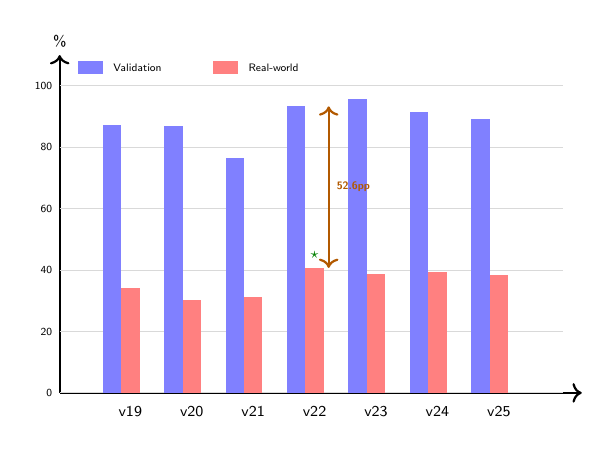
\begin{tikzpicture}[scale=0.78, transform shape]
    \begin{scope}
        \draw[thick, ->] (0,0) -- (8.5,0);
        \draw[thick, ->] (0,0) -- (0,5.5) node[above, font=\scriptsize\sffamily] {\%};
        \foreach \y/\label in {0/0, 1/20, 2/40, 3/60, 4/80, 5/100} {
            \draw[gray!30] (0,\y) -- (8.2,\y);
            \node[left, font=\tiny\sffamily] at (0,\y) {\label};
        }
        \def\bw{0.3}
        % Validation bars (blue)
        \foreach \x/\val in {1/4.365, 2/4.345, 3/3.825, 4/4.665, 5/4.78, 6/4.575, 7/4.455} {
            \fill[blue!50] (\x-\bw,0) rectangle (\x,\val);
        }
        % Real-world bars (red)
        \foreach \x/\val in {1/1.71, 2/1.515, 3/1.56, 4/2.035, 5/1.93, 6/1.965, 7/1.915} {
            \fill[red!50] (\x,0) rectangle (\x+\bw,\val);
        }
        % Gap arrow for v22
        \draw[<->, thick, orange!70!black] (4+\bw+0.08, 2.035) -- (4+\bw+0.08, 4.665)
            node[midway, right, font=\tiny\sffamily\bfseries, text=orange!70!black] {52.6pp};
        % X labels
        \foreach \x/\label in {1/v19, 2/v20, 3/v21, 4/v22, 5/v23, 6/v24, 7/v25} {
            \node[below, font=\scriptsize\sffamily] at (\x+\bw/2, -0.1) {\label};
        }
        \node[font=\scriptsize, text=green!50!black] at (4+\bw/2, 2.25) {$\star$};
        % Legend
        \fill[blue!50] (0.3, 5.2) rectangle (0.7, 5.4);
        \node[right, font=\tiny\sffamily] at (0.75, 5.3) {Validation};
        \fill[red!50] (2.5, 5.2) rectangle (2.9, 5.4);
        \node[right, font=\tiny\sffamily] at (2.95, 5.3) {Real-world};
    \end{scope}
    \end{tikzpicture}
    \caption{Validation vs.\ real-world accuracy (v19--v25). The persistent $\sim$53pp gap shows that architecture changes aren't solving the generalization problem. Star marks best real-world model (v22).}
    \label{fig:gap}
\end{figure}

% ============================================================
% 7. DISCUSSION
% ============================================================
\section{Discussion}

\subsection{Lessons from 25 Versions}

Twenty-five versions is a lot of models. Here's what we took away from the experience.

\textbf{Simpler is usually better.} At three separate points in the project---v10 (ditching engineered features), v17 (stripping out confusion-aware loss), and v22 (dropping ArcFace)---removing complexity improved real-world performance. Our best model has 776K parameters. Compare that to the 4--5M from v7, the 7M models in v15--v18, or the 3.1M per stream in v23. When your training set is four signers, a smaller model that doesn't overfit to their quirks just works better.

\textbf{Don't trust validation accuracy.} This might be our single most important finding. Before we started testing on real signers at v19, validation accuracy was all we had to go on. It painted a very misleading picture. Version 23's record-setting 95.6\% validation translated to just 38.6\% in the real world---actually worse than v22, which scored 93.3\%/40.7\%. The roughly 53-point gap stayed stubbornly consistent no matter what we tried, confirming findings from Li et al.~\cite{li2020wlasl}, Sincan and Keles~\cite{sincan2020autsl}, and Desmond et al.~\cite{desmond2024}. If you're building an SLR system and only evaluating on a held-out signer from the same recording session, you're fooling yourself.

\textbf{Errors get shuffled, not fixed.} Confusion-aware penalties in v8 and v16, class boosting in v7, anti-attractor heads in v8/v16/v18---every time we tried to squash a specific confusion pattern, a new one popped up somewhere else. The underlying problem is that with only four unique signers, some classes genuinely look identical from the model's perspective. No amount of loss function engineering can create distinguishing information that isn't in the data.

\textbf{The GCN bet paid off, eventually.} Switching from hand-engineered features to a graph convolution approach in v10 felt like a leap of faith at the time. We gave up 100-plus carefully designed features on the hope that the network would learn its own spatial representations. It took 14 versions for that bet to fully pay off (v22, 93.3\% val versus v8's 83.7\%), but the GCN's inductive bias---that hands are best modeled as spatial graphs---turned out to be right for this task.

\textbf{Bugs are invisible until you look.} The v17 pipeline audit found 4 bugs, and v18 fixed 11 total. These weren't exotic issues---normalization that was quietly squashing values, SWA code that never ran, a temporal roll that wrapped incorrectly, an incomplete hand-swap implementation. They'd been silently degrading results for several versions, their effects hidden by other changes. The audit was more valuable than any architectural innovation we attempted.

\textbf{Numbers and words are different problems.} This became unmistakable from v24 onward. Hand-body spatial features helped words (which involve signing at distinctive body locations) but hurt numbers (which are all about hand shape regardless of where the hand is). Versions 24 and 25 both hit the best-ever word accuracy (49.4\%) while numbers languished at 25--27\%. Treating them as one unified problem obscured important dynamics.

\subsection{The Four-Signer Ceiling}

Seven architecturally diverse models (v19--v25), spanning 776K to 17.3M parameters and employing state-of-the-art domain generalization techniques (GRL, MixStyle, prototypical networks, multi-stream fusion, ArcFace, hand-body spatial features, temporal CutMix), all landed between 30\% and 41\% on real-world accuracy. McNemar's tests found no significant differences between any pair. LOSO cross-validation on v25 reached 94.7\%---confirming the architecture can learn the task---but real-world performance sat at 38.3\%.

We interpret this as a hard ceiling imposed by training on four unique signers. And the data audit reinforced this: what we'd recorded as five training signers was actually four, since two of the recordings were duplicates. The model transfers perfectly within the training distribution (LOSO 94.7\%) but can't handle the variation introduced by genuinely new people.

This matches what others have found. Guo et al.~\cite{guo2024fewshot} got 43.75\% on ASL with prototypical networks, and Desmond et al.~\cite{desmond2024} documented 20--40pp accuracy drops in signer-independent settings. Our roughly 40\% accuracy with 4 signers appears to be the expected performance level, not a KSL-specific problem.

\subsection{Diagnostic Findings}

The v25 diagnostic audit surfaced two issues worth highlighting. The duplicate signer discovery---byte-identical MD5 hashes for signers 2 and 3---means our effective training diversity was lower than we thought. We suspect this doesn't dramatically change the 4-signer-vs-real-world gap (the held-out validation signer was still unique), but it does mean the model saw less stylistic variation than intended.

The MediaPipe version mismatch (training data extracted with v0.10.14, evaluation with v0.10.5) introduces a subtle distribution shift at the feature extraction level. Minor version changes in MediaPipe can adjust landmark detection models, shifting coordinate outputs by small amounts. We haven't quantified the impact, but it's a free source of noise that future work should eliminate by re-extracting all data with a single MediaPipe version.

\subsection{Recommendations}

After 25 versions and roughly six months of development, here's what we'd tell someone starting a similar project:

\begin{enumerate}
    \item \textbf{Recruit more signers first.} Our results strongly suggest that 7--10 signers is the minimum for reasonable cross-signer generalization. No architectural trick we tried could compensate for having only four.
    \item \textbf{Test on unseen signers from day one.} We wasted versions v0 through v18 optimizing a metric (validation accuracy) that turned out to be nearly uncorrelated with real-world performance. If we'd started real-tester evaluation earlier, we'd have saved months.
    \item \textbf{Start with the simplest model that works.} A 776K-parameter ST-GCN beat or matched everything we threw at the problem, including models 22$\times$ its size. Complexity is a liability when training data is scarce.
    \item \textbf{Audit your pipeline before your architecture.} Bug fixes (v17--v18) and simplification (v17, v22) consistently outperformed novel loss functions, fusion strategies, and classification heads. The boring stuff matters most.
    \item \textbf{Check your data.} We didn't discover our duplicate signers or MediaPipe version mismatch until version 25. Both could have been caught much earlier with a routine data audit.
    \item \textbf{Publish negative results.} Our multi-stream fusion, prototypical classification, MixStyle, ArcFace, hand-body features, and CutMix experiments didn't work. Knowing that saves other researchers from rediscovering the same dead ends.
\end{enumerate}

\subsection{Limitations}

The test set is small---140 videos from 3 signers. Our vocabulary covers only 30 isolated signs, and the system uses only manual features, ignoring facial expressions and head movements that carry grammatical meaning in KSL. Results for v0--v14 lack systematic validation measurements, making it impossible to know exactly when certain capabilities emerged. The platform migration from Modal to Alpine introduced confounding variables we couldn't fully control for. The MediaPipe version mismatch between training and evaluation data adds an unquantified noise floor. And we can't prove that more signers would break the ceiling without actually collecting that data---though the literature and our LOSO results give us strong reason to believe they would.

% ============================================================
% 8. CONCLUSION
% ============================================================
\section{Conclusion}

This paper tells the story of 25 model versions built over six months, tracing the first automated Kenya Sign Language recognition system from a bare-bones Transformer prototype to a graph convolutional architecture that handles the task well within its training distribution but struggles with new signers. Our best model overall---a compact 776K-parameter ST-GCN with gradient reversal---hits 93.3\% validation and 40.7\% on unseen signers. Version 25, the latest iteration, pushed word recognition to its highest point yet (49.4\%) using hand-to-body spatial features, but this came at the cost of number recognition (27.1\%), and overall accuracy (38.3\%) still didn't surpass v22.

The central takeaway is this: when you only have four training signers, no amount of architectural creativity will get you past roughly 40\% accuracy on new people. We tried multi-stream fusion, prototypical classification, domain randomization with MixStyle, ArcFace margins, hand-body spatial features, temporal CutMix, confusion-aware loss functions, and test-time augmentation. None of it moved the needle meaningfully. LOSO cross-validation confirms the model can reach 94.7\% within the training distribution, putting the entire 56-point gap squarely on out-of-distribution signer variation. Meanwhile, a data audit revealed that our training set had fewer unique signers than we thought and a MediaPipe version mismatch between training and evaluation---issues that only came to light when we stopped trying to improve the architecture and started scrutinizing the data.

On the other hand, simplification, bug fixing, and pipeline auditing proved consistently more valuable than adding complexity. That's a less glamorous finding, but we think it's a more useful one.

We chose to report this complete 25-version journey---including the 19 versions that came before our best result and the 3 that failed to improve on it---because the machine learning community needs more papers that show the full picture. The false starts, the techniques that didn't work, the bugs that went unnoticed for weeks---that's what real development looks like, and it's what other practitioners can actually learn from. Future work should focus on expanding signer diversity, extending to continuous signing, and exploring transfer learning from larger sign language datasets.

% ============================================================
% REFERENCES
% ============================================================
\bibliographystyle{IEEEtran}
\begin{thebibliography}{35}

\bibitem{ai4ksl2024}
AI4KSL Project, ``Creating a digital open-access Kenya Sign Language dataset,'' \textit{arXiv:2410.18295}, 2024.

\bibitem{aiman2023}
U.~Aiman and T.~Ahmad, ``Angle based hand gesture recognition using graph convolutional network,'' \textit{Comp. Anim. Virtual Worlds}, vol.~35, no.~1, 2023.

\bibitem{amukasa2021}
Amukasa, ``Translating the Kenyan Sign Language with Deep Learning,'' Tech. report, 2021.

\bibitem{anithadevi2025}
N.~Anithadevi \textit{et al.}, ``MediaPipe-LSTM-Enhanced Framework for Real-Time Dynamic SLR,'' \textit{Eng. Reports}, vol.~7, no.~7, 2025.

\bibitem{chen2021ctrgcn}
Y.~Chen \textit{et al.}, ``Channel-wise Topology Refinement Graph Convolution for Skeleton-Based Action Recognition,'' in \textit{Proc. ICCV}, 2021.

\bibitem{deng2019arcface}
J.~Deng \textit{et al.}, ``ArcFace: Additive Angular Margin Loss for Deep Face Recognition,'' in \textit{Proc. CVPR}, 2019.

\bibitem{desmond2024}
D.~Desmond \textit{et al.}, ``Signer-independent sign language recognition: A comprehensive review,'' 2024.

\bibitem{dodge2019}
J.~Dodge \textit{et al.}, ``Show Your Work: Improved Reporting of Experimental Results,'' in \textit{Proc. EMNLP}, 2019.

\bibitem{ganin2016domain}
Y.~Ganin \textit{et al.}, ``Domain-Adversarial Training of Neural Networks,'' \textit{JMLR}, vol.~17, no.~59, pp.~1--35, 2016.

\bibitem{guo2024fewshot}
Guo \textit{et al.}, ``Data-Efficient ASL Recognition via Few-Shot Prototypical Networks,'' \textit{arXiv:2512.10562}, 2024.

\bibitem{hasan2025}
A.~Hasan \textit{et al.}, ``Bangla Sign Language Recognition With Multimodal Deep Learning Fusion,'' \textit{Eng. Reports}, vol.~7, no.~4, 2025.

\bibitem{hochreiter1997}
S.~Hochreiter and J.~Schmidhuber, ``Long Short-Term Memory,'' \textit{Neural Computation}, vol.~9, no.~8, pp.~1735--1780, 1997.

\bibitem{huang2022}
J.~Huang \textit{et al.}, ``CNN-BiLSTM sign language recognition,'' \textit{Electronics}, 2022.

\bibitem{ioffe2015}
S.~Ioffe and C.~Szegedy, ``Batch Normalization: Accelerating Deep Network Training,'' in \textit{Proc. ICML}, 2015.

\bibitem{khosla2020supcon}
P.~Khosla \textit{et al.}, ``Supervised Contrastive Learning,'' in \textit{Proc. NeurIPS}, 2020.

\bibitem{koller2015}
O.~Koller \textit{et al.}, ``Continuous sign language recognition: Towards large vocabulary statistical recognition systems,'' \textit{CVIU}, 2015.

\bibitem{kolawole2024augmentation}
Kolawole \textit{et al.}, ``Enhancing Human Action Recognition with 3D Skeleton Data,'' \textit{Electronics}, vol.~13, no.~4, 2024.

\bibitem{li2020wlasl}
D.~Li \textit{et al.}, ``Word-level Deep Sign Language Recognition from Video,'' in \textit{Proc. WACV}, 2020.

\bibitem{lin2017focal}
T.-Y.~Lin \textit{et al.}, ``Focal Loss for Dense Object Detection,'' in \textit{Proc. ICCV}, 2017.

\bibitem{lipton2019}
Z.~C.~Lipton and J.~Steinhardt, ``Troubling Trends in Machine Learning Scholarship,'' \textit{Queue}, vol.~17, no.~1, 2019.

\bibitem{liu2020msg3d}
Z.~Liu \textit{et al.}, ``Disentangling and Unifying Graph Convolutions for Skeleton-Based Action Recognition,'' in \textit{Proc. CVPR}, 2020.

\bibitem{loshchilov2017cosine}
I.~Loshchilov and F.~Hutter, ``SGDR: Stochastic Gradient Descent with Warm Restarts,'' in \textit{Proc. ICLR}, 2017.

\bibitem{loshchilov2019adamw}
I.~Loshchilov and F.~Hutter, ``Decoupled Weight Decay Regularization,'' in \textit{Proc. ICLR}, 2019.

\bibitem{moustafa2023}
A.~M.~Moustafa \textit{et al.}, ``Integrated Mediapipe with a CNN Model for Arabic SLR,'' \textit{J. Elec. Comp. Eng.}, 2023.

\bibitem{muller2019}
R.~M\"{u}ller \textit{et al.}, ``When Does Label Smoothing Help?,'' in \textit{Proc. NeurIPS}, 2019.

\bibitem{oyedotun2017}
O.~K.~Oyedotun and A.~Khashman, ``Deep learning in vision-based static hand gesture recognition,'' \textit{Neural Computing and Applications}, 2017.

\bibitem{pigou2015}
L.~Pigou \textit{et al.}, ``Sign Language Recognition Using Convolutional Neural Networks,'' in \textit{Proc. ECCV Workshops}, 2015.

\bibitem{pu2024signer}
J.~Pu \textit{et al.}, ``Improving CSLR with Consistency Constraints and Signer Removal,'' \textit{ACM TOMM}, 2024.

\bibitem{robert2023review}
E.~J.~Robert and H.~J.~Duraisamy, ``A review on computational methods based automated SLR system,'' \textit{CCPE}, vol.~35, no.~9, 2023.

\bibitem{shi2019twostreamAGCN}
L.~Shi \textit{et al.}, ``Two-Stream Adaptive Graph Convolutional Networks for Skeleton-Based Action Recognition,'' in \textit{Proc. CVPR}, 2019.

\bibitem{sincan2020autsl}
O.~M.~Sincan and H.~Y.~Keles, ``AUTSL: A Large Scale Multi-Modal Turkish Sign Language Dataset and Baseline Methods,'' \textit{IEEE Access}, 2020.

\bibitem{snell2017prototypical}
J.~Snell \textit{et al.}, ``Prototypical Networks for Few-shot Learning,'' in \textit{Proc. NeurIPS}, 2017.

\bibitem{srivastava2014}
N.~Srivastava \textit{et al.}, ``Dropout: A Simple Way to Prevent Neural Networks from Overfitting,'' \textit{JMLR}, vol.~15, pp.~1929--1958, 2014.

\bibitem{szegedy2016}
C.~Szegedy \textit{et al.}, ``Rethinking the Inception Architecture for Computer Vision,'' in \textit{Proc. CVPR}, 2016.

\bibitem{yan2018stgcn}
S.~Yan \textit{et al.}, ``Spatial Temporal Graph Convolutional Networks for Skeleton-Based Action Recognition,'' in \textit{Proc. AAAI}, 2018.

\bibitem{zhang2018mixup}
H.~Zhang \textit{et al.}, ``mixup: Beyond Empirical Risk Minimization,'' in \textit{Proc. ICLR}, 2018.

\bibitem{zhang2020mediapipe}
F.~Zhang \textit{et al.}, ``MediaPipe Hands: On-device Real-time Hand Tracking,'' \textit{arXiv:2006.10214}, 2020.

\bibitem{zhou2021mixstyle}
K.~Zhou \textit{et al.}, ``Domain Generalization with MixStyle,'' in \textit{Proc. ICLR}, 2021.

\end{thebibliography}

\end{document}
